\documentclass{beamer}
\usepackage[utf8x]{inputenc}
\usepackage[english, greek]{babel}
\usepackage{svCognAC, soul, array, enumerate, fancyvrb, graphicx, hyperref, listings, multicol, multirow, url, xcolor, xfrac}
\usepackage{tikz, tikzsymbols, tipa}

\usetikzlibrary{arrows.meta}

\newcommand{\red}[1]{\textcolor{red}{#1}}
\renewcommand{\;}{\hspace{0.25em}}

\mode<presentation>{}

\title[\LaTeX\;workshop]{
  \LaTeX\;workshop}

\author[Arjan Wildhagen]{
  Arjan Wildhagen \\ \vspace{3.5cm}
  }
  
\institute[]{}

\date[\today]{\today}

\begin{document}
\selectlanguage{english}
\begin{frame}
	\titlepage
	\begin{tikzpicture}[overlay]
		\node[anchor=south west] at (0,0) {};
		\node[xshift=15mm, yshift=18mm, anchor=south west] at (0,0) {
\includegraphics[width=7cm]{Images/LatexWorkshop}};
	\end{tikzpicture}
\end{frame}

\section{What is \LaTeX}
\begin{frame}
	\frametitle{What is \LaTeX}
	\begin{multicols}{2}
		\begin{itemize}
			\item \TeX\;invented by Donald Knuth in 1977
			\begin{itemize}
				\item[\textendash] /\textipa{`tEx}/ or /\textipa{`tEk}/, from the word {\selectlanguage{greek}téχnh} meaning \textit{art} or \textit{craft}, root of \textit{technical}
			\end{itemize}
			\item Extended to \LaTeX\;by Leslie Lamport in 1984
			\begin{itemize}
				\item[\textendash] /\textipa{la`tEx}/ or /\textipa{lei`tEk}/
			\end{itemize}
		\end{itemize}
		\hfill\columnbreak
		\begin{figure}
			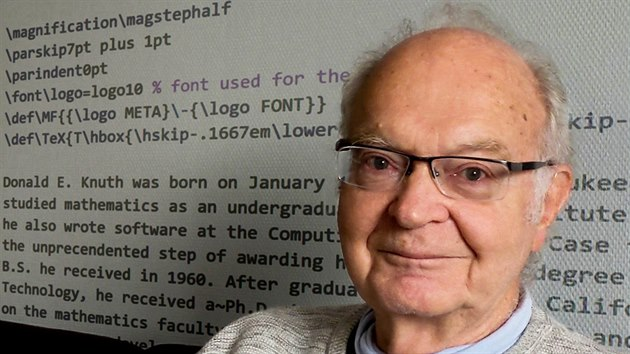
\includegraphics[width=4cm]{Images/DonaldKnuth}
			\\[2mm]
			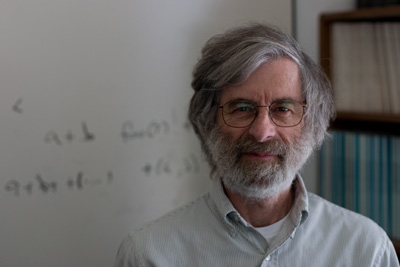
\includegraphics[width=4cm]{Images/LeslieLamport}
		\end{figure}
	\end{multicols}
\end{frame}

\begin{frame}[fragile]
\frametitle{\LaTeX $>$ Word}
\LaTeX\;uses dynamic programming to minimize spacing.

\begin{multicols}{2}
\textbf{Microsoft Word}
\begin{verbatim}
hey hey hey
hey
stupidbitch
\end{verbatim}
\phantom{\phantom{w}\quad\tikzsymbolsuse{Sadey}[4.4]}
\columnbreak

\textbf{\LaTeX}
\begin{verbatim}
hey hey
hey hey
stupidbitch
\end{verbatim}
\phantom{\phantom{w}\tikzsymbolsuse{Smiley}[4.4]}
\end{multicols}

\end{frame}

\begin{frame}[fragile]
\frametitle{\LaTeX $>$ Word}
\LaTeX\;uses dynamic programming to minimize spacing.

\begin{multicols}{2}
\textbf{Microsoft Word}
\begin{verbatim}
hey hey hey
hey
stupidbitch
\end{verbatim}
{\phantom{w}\quad\tikzsymbolsuse{Sadey}[3]}
\columnbreak

\textbf{\LaTeX}
\begin{verbatim}
hey hey
hey hey
stupidbitch
\end{verbatim}
{\phantom{w}\tikzsymbolsuse{Smiley}[3]}
\end{multicols}

\end{frame}

\section{Why use \LaTeX}
\begin{frame}
\frametitle{Pros and Cons}
	\begin{multicols}{2}
	Pros:
	\begin{itemize}
		\item<2-> Beautiful typesetting
		\item<3-> Mathematical support
		\item<4-> Very customizable
		\item<5-> Lots of (academic) support
		\item<6-> Easy footnotes, references, indices, etc.
		\item<7-> Tex file holds all info of document (given that packages are available)
		\item<8-> Very robust
	\end{itemize}
	\vfill
	\columnbreak
	Cons
	\begin{itemize}
		\item<9-> Maybe difficult to get into
		\item<10-> Very customizable, but how do you do it?
		\item<11-> Frustrating placements or creations
		\item<12-> Sometimes very hard to get specific layout
	\end{itemize}
\end{multicols}

\end{frame}

\section{How to \LaTeX}

\begin{frame}
	\frametitle{How to \LaTeX}
	5 Levels of \LaTeX\; understanding
	\begin{itemize}
		\item<2-> Beginner
		\item<3-> Intermediate
		\item<4-> Advanced
		\item<5-> Expert
		\item<6-> \st{Godlike} Dark side of \LaTeX
	\end{itemize}
\end{frame}

\begin{frame}
	\frametitle{Levels of \LaTeX}
	5 Levels of \LaTeX\; understanding
	\begin{itemize}
		\item Beginner
		\item Intermediate
		\item \st{Advanced}
		\item \st{Expert}
		\item \st{Godlike} \st{Dark side of \LaTeX}
	\end{itemize}
\end{frame}

\begin{frame}
\frametitle{Where to \LaTeX?}
	\centering
	UI's
	\begin{multicols}{3}
		\hspace{-.8cm}\textbf{Linux}
		\begin{itemize}
			\item TeXLive
			\item Gummi
			\item Kile
			\item Latexila
		\end{itemize}
		\vfill
		\columnbreak
		\textbf{Windows}
		\begin{itemize}
			\item MikTex
			\item TexnicCenter
			\item WinEdt
			\item TexStudio (works on all platforms)
		\end{itemize}
		\vfill
		\columnbreak
		\hspace{-0.5cm}\textbf{MacOS}
		\begin{itemize}
			\item MacTex
			\item TexShop
			\item Texnicle
			\item Archimedes
		\end{itemize}
		\vfill
		\columnbreak
	\end{multicols}
	\vspace{5mm}
\end{frame}

\begin{frame}
\frametitle{Where to \LaTeX?}
	\centering
	UI's
	\begin{multicols}{3}
		\hspace{-.8cm}\textbf{Linux}
		\begin{itemize}
			\item TeXLive
			\item Gummi
			\item Kile
			\item Latexila
		\end{itemize}
		\vfill
		\columnbreak
		\textbf{Windows}
		\begin{itemize}
			\item MikTex
			\item TexnicCenter
			\item WinEdt
			\item TexStudio (works on all platforms)
		\end{itemize}
		\vfill
		\columnbreak
		\hspace{-0.5cm}\textbf{MacOS}
		\begin{itemize}
			\item MacTex
			\item TexShop
			\item Texnicle
			\item Archimedes
		\end{itemize}
		\vfill
		\columnbreak
	\end{multicols}
	
	\begin{tikzpicture}[overlay]
		\node[anchor=south west] at (0,0) {};
		\node[xshift=-62mm, yshift=8mm, anchor=south west] at (0,0) {
\includegraphics[width=12cm]{Images/Overleaf}};
	\end{tikzpicture}

\end{frame}

\begin{frame}
\frametitle{Files}
	Filename extensions
	\begin{itemize}
		\item .tex\quad standard \TeX\; file
		\item .bib\quad bibliography file
		\item .bst\quad bibliography formatting file
		\item .cls\hspace{0.86em} class file
		\item .sty\hspace{0.76em} style file
		\item And more...
	\end{itemize}
\end{frame}

\begin{frame}[fragile]
\frametitle{Hello world!}
	Our first \LaTeX\; document!
	\begin{multicols}{2}
	\begin{Verbatim}[frame=single]
\documentclass{article}
\begin{document}
Hello World!
\end{document}
	\end{Verbatim}
	\vfill
	\columnbreak
	\begin{Verbatim}[frame=single]
Hello World!



	\end{Verbatim}
	\end{multicols}
	\phantom{\begin{tikzpicture}[overlay]
		\node[anchor=south west] at (0,0) {};
		\node[xshift=-62mm, yshift=8mm, anchor=south west] at (0,0) {
\includegraphics[width=12cm]{Images/RedArrow}};
	\end{tikzpicture}}
\end{frame}

\begin{frame}[fragile]
\frametitle{Hello world!}
	Our first \LaTeX\; document!
	\begin{multicols}{2}
	\begin{Verbatim}[frame=single]
\documentclass{article}
\begin{document}
Hello World!
\end{document}
	\end{Verbatim}
	\vfill
	\columnbreak
	\begin{Verbatim}[frame=single]
Hello World!



	\end{Verbatim}
	\end{multicols}
	\begin{tikzpicture}[overlay]
		\node[anchor=south west] at (0,0) {};
		\node[text width = 6cm] at (7.5,5) {\red{Many different options! (proc, book, report, slides, beamer, etc.)}};
		\draw[-{Triangle[width=18pt,length=8pt, color=red]}, line width=10pt, color=red](4, 5) -- (2, 3);
	\end{tikzpicture}
\end{frame}

\begin{frame}[fragile]
\frametitle{Hello world!}
	Our first \LaTeX\; document!
	\begin{multicols}{2}
	\begin{Verbatim}[frame=single]
\documentclass{article}
\begin{document}
Hello World!
\end{document}
	\end{Verbatim}
	\vfill
	\columnbreak
	\begin{Verbatim}[frame=single]
Hello World!



	\end{Verbatim}
	\end{multicols}
	\begin{tikzpicture}[overlay]
		\node[anchor=south west] at (0,0) {};
		\draw[-{Triangle[width=18pt,length=8pt, color=red]}, line width=10pt, color=red](3, 4.5) -- (1, 2.5);
		\draw[-{Triangle[width=18pt,length=8pt, color=red]}, line width=10pt, color=red](3, -1.5) -- (0.75, 1.1);
		\node[text width = 8cm] at (7.5,-1) {\red{Everything in front of \textbackslash begin\{document\} is called the preamble and will not show up in the document.}};
	\end{tikzpicture}
\end{frame}

\begin{frame}
\frametitle{Reserved characters}
	\LaTeX\;has some characters reserved where typing them evokes a functionality\\[2mm]
These chars are: \# \$ \% \^{} \& \_ \{ \} \~{} \textbackslash
\end{frame}

\begin{frame}[fragile]
\frametitle{Packages}
Packages can be treated as libraries in other programming languages (e.g. Java or Python). They can be invoked by typing the usepackage command, and possible parameters:\\[2mm]
\begin{Verbatim}[frame=single]
\usepackage[parameters]{package_name}
\end{Verbatim}
\vspace{2.05cm}
\end{frame}

\begin{frame}[fragile]
\frametitle{Packages}
Packages can be treated as libraries in other programming languages (e.g. Java or Python). They can be invoked by typing the usepackage command, and possible parameters:\\[2mm]
\begin{Verbatim}[frame=single]
\usepackage[parameters]{package_name}
\end{Verbatim}
\textit{Hint: You can concatenate multiple packages if they do not need a parameter. E.g.:}\\[2mm]
\begin{Verbatim}[frame=single]
\usepackage{package_name1, package_name2, ...}
\end{Verbatim}
\end{frame}

\begin{frame}
\frametitle{Packages}
Useful packages:
\begin{itemize}
\item amsmath, amssymb, amsthm, mathtools, xfrac
\item caption, float, graphicx, tikz
\item comment, enumerate, geometry, hyperref, verbatim
\item array, babel, hyperref, listings, xcolor
\item many many more (to be found at the \href{https://www.ctan.org/}{\red{CTAN website}})
\end{itemize}
\end{frame}

\begin{frame}
\frametitle{Some more basics}
Chapters/sections have a level of appereance. Parts and chapters are usually only used in books\\
\begin{multicols}{2}
\begin{tabular}{|l c|}
\hline
Command & Level\\
\hline
\textbackslash part & -1\\
\textbackslash chapter & 0\\
\textbackslash section & 1\\
\textbackslash subsection & 2\\
\textbackslash subsubsection & 3\\
\textbackslash paragraph & 4\\
\textbackslash subparagraph & 5\\
\hline

\end{tabular}
\vfill
\columnbreak
If the number in front of the section/paragraph is unwanted, a * can be added after the command to remove this enumeration.\\[2mm]
\textbackslash section\{example\}$\rightarrow$\textbf{1 Example}\\[1mm]
\textbackslash section*\{example\}$\rightarrow$\textbf{Example}
\end{multicols}
\end{frame}

\begin{frame}
\frametitle{Spacing}
(Horizontal) spacing is defined with multiple commands, and a generic one. Basic lengths are points (pt), millimeter (mm), centimeter (cm), inch (in), height of an x in current font (ex) and width of an M in current font (em). From small to large:\\[2mm]
\begin{multicols}{2}
\begin{tabular}{|l c|}
\hline
Command & space\\
\hline
\textbackslash ! & -\sfrac{3}{18} em\\
\textbackslash , & \sfrac{3}{18} em\\
\textbackslash $>$ or \textbackslash : & \sfrac{4}{18} em\\
\textbackslash ; & \sfrac{5}{18} em\\
\textbackslash enspace & \sfrac{1}{2} em\\
\textbackslash quad & 1 em\\
\textbackslash qquad & 2 em\\
\textbackslash hspace\{\dots\} & \dots\\
\hline

\end{tabular}
\vfill
\columnbreak
The command \textbackslash linespread\{\dots\} changes the whitespace between lines in the document. \textbackslash linespread\{1\} is standard, \textbackslash linespread\{1.6\} is doubled whitespace.
\end{multicols}
\end{frame}

\begin{frame}
\frametitle{Font sizes}
Font sizes of the whole document can be changed as a parameter of the documentclass command, e.g. \textbackslash documentclass[12pt]\{article\}. Different fonts are possible, search for the correct package on Google. Sizing fonts from small to large (assuming the original fontsize is 11pt):\\[2mm]
\begin{multicols}{2}
\begin{tabular}{|l c|}
\hline
Command & size\\
\hline
\textbackslash tiny & 6 pt\\
\textbackslash scriptsize & 8 pt\\
\textbackslash footnotesize & 9 pt\\
\textbackslash small & 10 pt\\
\textbackslash normalsize & 10.95 pt\\
\hline

\end{tabular}
\vfill
\columnbreak
\begin{tabular}{|l c|}
\hline
Command & size\\
\hline
\textbackslash large & 12 pt\\
\textbackslash Large & 14.4 pt\\
\textbackslash LARGE & 17.28 pt\\
\textbackslash huge & 20.74\\
\textbackslash Huge & 24.88\\
\hline

\end{tabular}
\end{multicols}
\end{frame}

\begin{frame}
\frametitle{Important distinction}
\centering
\begin{tabular}{p{4.5cm} p{0.5cm} p{4.5cm}}
\textbf{Groups/Switches} & vs & \textbf{Environment}\\[2mm]
Defines something until the group is ended, or for the whole document & & Only applies to the code written in between the \textbackslash begin\{\} and \textbackslash end\{\} \newline\\
\textbackslash centering is a switch \newline \{\textbackslash centering\} creates a local scope/group, or with \textbackslash bgroup \textbackslash centering \textbackslash egroup& & \textbackslash begin\{centering\}\dots\newline \textbackslash end\{centering\} is an environment\\
& & \\
\end{tabular}
\red{Not every switch can be transformed into an environment, and vice versa!}
\end{frame}

\begin{frame}
\frametitle{Almost there}
{\Huge So, now lets dive into some examples}
\end{frame}

\begin{frame}[t, fragile]
\frametitle{Tables}
Tables are one of the most frustrating things most users experience, but you are not alone!\\[1mm]
Use \url{https://www.tablesgenerator.com/} to help you out a lot.\\[1mm]
There are many environments that help with tables:
	\begin{itemize}
		\item tabular, tabular*, tabularx, tabulary, array, \dots
	\end{itemize}
In essence a table is easily defined with: 
	\begin{Verbatim}[frame=single]
\begin{tabular}{nr of columns and specs}
Cell1.1 & Cell1.2 & ... \\ ← New row!
Cell2.1 & Cell2.2 & ... \\ ← New row!
\end{tabular}
	\end{Verbatim}
At \textit{nr of coumns and specs} you can define columns and their text alignment. \{l c r\} means 3 columns, the first is left aligned, the second is centered, the third one is right aligned.
\end{frame}

\begin{frame}[t, fragile]
\frametitle{Tables}
We can also specify borders and merge cells.

\begin{Verbatim}[frame=single]
\begin{tabular}{c||l|r}
\hline
\multirow{2}{*}{Merged cell!} & Well & hello\\
 & there & \multicolumn{1}{c|}{General} \\
\cline{2-3}
\multicolumn{2}{c|}{Merged cell!} & Kenobi
\end{tabular}
\end{Verbatim}
\begin{centering} 
	$\downarrow$ produces $\downarrow$\\
	\phantom{w}\hspace{2cm}
	\begin{tabular}{c||l|r}
		\hline
		\multirow{2}{*}{Merged cell!} & Well & hello\\
 		& there & \multicolumn{1}{c|}{General} \\
		\cline{2-3}
		\multicolumn{2}{c|}{Merged cell!} & Kenobi
	\end{tabular}
\end{centering}
\end{frame}

\begin{frame}[t, fragile]
\frametitle{Lists}
To simply list a couple of items, the following should be good (you can also change the symbol):
\begin{multicols}{2}
\begin{Verbatim}[frame=single]
\begin{itemize}
 \item Nr.1
 \item[\textendash] Nr.2
 \item[$\lambda$] Nr.3
\end{itemize}
\end{Verbatim}
\vfill\columnbreak
\phantom{w}\vspace{-2mm}
\begin{itemize}
	\item Nr.1
	\item[\textendash] Nr.2
	\item[$\lambda$] Nr.3
\end{itemize}
\end{multicols}
\end{frame}

\begin{frame}[t, fragile]
\frametitle{Lists}
Or use the enumerate package to help you with ordering lists:
\begin{multicols}{2}
\begin{Verbatim}[frame=single]
\begin{enumerate}[a)]
 \item Nr.1
 \item Nr.2
 \item[$\eta$] Nr.3
\end{enumerate}
\end{Verbatim}
\vfill\columnbreak
\phantom{w}\vspace{-2mm}
\begin{enumerate}[a)]
 \item[a)] Nr.1
 \item[b)] Nr.2
 \item[$\eta$] Nr.3
\end{enumerate}
\end{multicols}
\end{frame}

\begin{frame}[t, fragile]
\frametitle{Figures}
Using figures is best with the graphicx package. The standard creation of a figure is as follows:
\begin{multicols}{2}
\begin{Verbatim}[frame=single]
\begin{figure}[floats]
 \centering
 \includegraphics →
→[parameters]{filepath}
 \caption{Caption}
 \label{fig:my_fig}
\end{figure}
\end{Verbatim}
\vfill\columnbreak
\begin{figure}
 \centering
 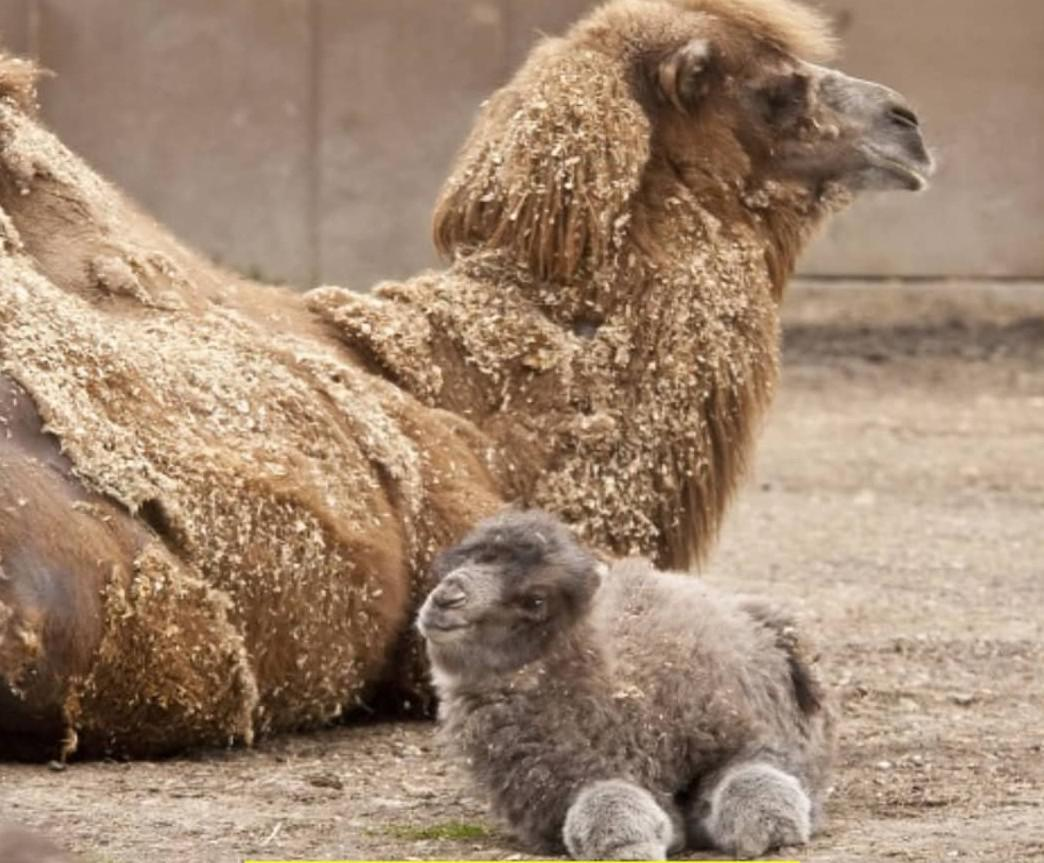
\includegraphics[width=4cm]{Images/BabyCamel}
 \caption{Baby Camel}
 \label{fig:my_fig}
\end{figure}
\end{multicols}
\end{frame}

\begin{frame}
\frametitle{Floats}
Determine where you want your figure (or rather floating object) to be, if the compiler is not doing a good job at it (\LaTeX\; automatically determines the best position). There are multiple floats available:

\begin{itemize}
	\item h\quad Place the object (\textit{approximately}) at this point
	\item t\hspace{3.1mm} Place the object at the top of the page
	\item b\quad Place the object at the bottom of the page
	\item p\quad Place the object on a special page for floating objects only
	\item !\hspace{3.1mm} Override internal parameters
	\item H\hspace{1.8mm} Place the object precisely at this point (same as !ht)
\end{itemize}
\end{frame}

\begin{frame}[t, fragile]
\frametitle{Labeling}
Create easy references to everything with a label. These references are dynamic, meaning that it will always refer to that specific label. This works for any floating object (\textit{Note: The label command appears after the caption command!)}
\begin{Verbatim}[frame=single]
Creating a label:
 \label{fig:my_label}

Creating a reference:
 \ref{fig:my_label)
\end{Verbatim}

\textit{Hint: Use the hyperref package to be able to click on the references and jump to the right object.}
\end{frame}

\begin{frame}[t, fragile]
\frametitle{Math mode}
Math mode allows multiple symbols, and all text is always in italics. Enter and leave math mode with \$, and create highlighted equations with \$\$, or with \textbackslash[ \dots \textbackslash]. Example:
\begin{Verbatim}[frame=single]
\[\sum_{n=0}^{\infty}\dfrac{1}{n^2} 
    = \dfrac{\pi^2}{6}\]
\end{Verbatim}
Produces
\[\sum_{n=0}^{\infty}\dfrac{1}{n^2} = \dfrac{\pi^2}{6}\]
\end{frame}

\begin{frame}[t, fragile]
\frametitle{Math mode}
The equation or align environment also allow highlighted equations, and the align environment also supports vertical alignment of specific characters (e.g. =):
\begin{Verbatim}[frame=single]
\begin{align}
 f(x) &= x\cdot y\\
&= y\cdot x
\end{align}
\end{Verbatim}
Which produces:
\begin{align}
 f(x) &= x\cdot y\\
&= y\cdot x
\end{align}
\end{frame}

\begin{frame}
\frametitle{Error handeling}
Some basic errors and what they mean:
\begin{tabular}{|p{3cm}| p{7cm}|}
\hline
Undefined control sequence & Used a command that does not exist\\
Underfull hbox & \LaTeX\; can't fill the whole line, usually to be ignored\\
Overfull hbox & \LaTeX\; tries to fit too much on 1 line, can also be ignored usually\\
Too many \}'s & There are too many \}'s in the document\\
Runaway argument & There are too little \}'s in the document\\
Missing \$ inserted & Either you used a command that should be in math mode, or math mode is never closed.\\
\hline
\end{tabular}
\end{frame}

\begin{frame}
\frametitle{Useful commands}
Here are some useful commands!
\begin{itemize}
	\item \textbackslash\textbackslash[length] → new line (no given length gives default height)
	\item \textbackslash newpage → Creates a new page
	\item \% → Comments one line of code
	\item \textbackslash newcommand\{\textbackslash comment\}[2]\{\#2\} → with the comment package this allows to easily comment multiple lines (add this before the start of the document)
	\item \textbackslash usepackage[a4paper, margin=3cm]\{geometry\} → Creating a bigger space on a page to work with
\end{itemize}
\end{frame}

\begin{frame}
\frametitle{What now?}
Use \url{http://detexify.kirelabs.org/classify.html} to help finding symbols\\[2mm]
Practise! As is with programming, 80\% is knowing how to search Google and extract information from Stack Overflow\\[2mm]
These slides, as the workshop file, can be found on my Github account where also (in the very near future) tutorials can be found for each level of understanding \LaTeX\; (link: \url{https://arjan-w.github.io/LaTeXHelp/})
\end{frame}

\end{document}
















